\documentclass[border=7pt]{standalone}
\usepackage{amsmath,amssymb}
\usepackage{tikz}
\usetikzlibrary{calc,positioning,arrows.meta,shapes.geometric,fit,backgrounds}

% =====================================================================
% Academic Figure Skill — Nature/Cell/Science Semantic Color Palette
% Fig. 3: Mid-Level Tactical Clustering, Extensible Guidance Interface &
%         FiLM Cluster-Conditioned Shared GRU-MAPPO (QA Polished)
% =====================================================================
\definecolor{cBlue}{HTML}{2166AC}
\definecolor{cBlueMid}{HTML}{4393C3}
\definecolor{cBlueBg}{HTML}{F0F6FC}

\definecolor{cGreen}{HTML}{1B7837}
\definecolor{cGreenMid}{HTML}{5AAE61}
\definecolor{cGreenBg}{HTML}{EFF8F1}

\definecolor{cOrange}{HTML}{B35806}
\definecolor{cOrangeMid}{HTML}{E08214}
\definecolor{cOrangeBg}{HTML}{FEF6EC}

\definecolor{cRed}{HTML}{B2182B}
\definecolor{cRedMid}{HTML}{D6604D}
\definecolor{cRedBg}{HTML}{FDF2F2}

\definecolor{cPurple}{HTML}{762A83}
\definecolor{cPurpleBg}{HTML}{F7F1FA}

\definecolor{cInk}{HTML}{1E293B}
\definecolor{cMuted}{HTML}{475569}
\definecolor{cGray}{HTML}{94A3B8}
\definecolor{cLine}{HTML}{CBD5E1}
\definecolor{cPanel}{HTML}{F8FAFC}

\begin{document}
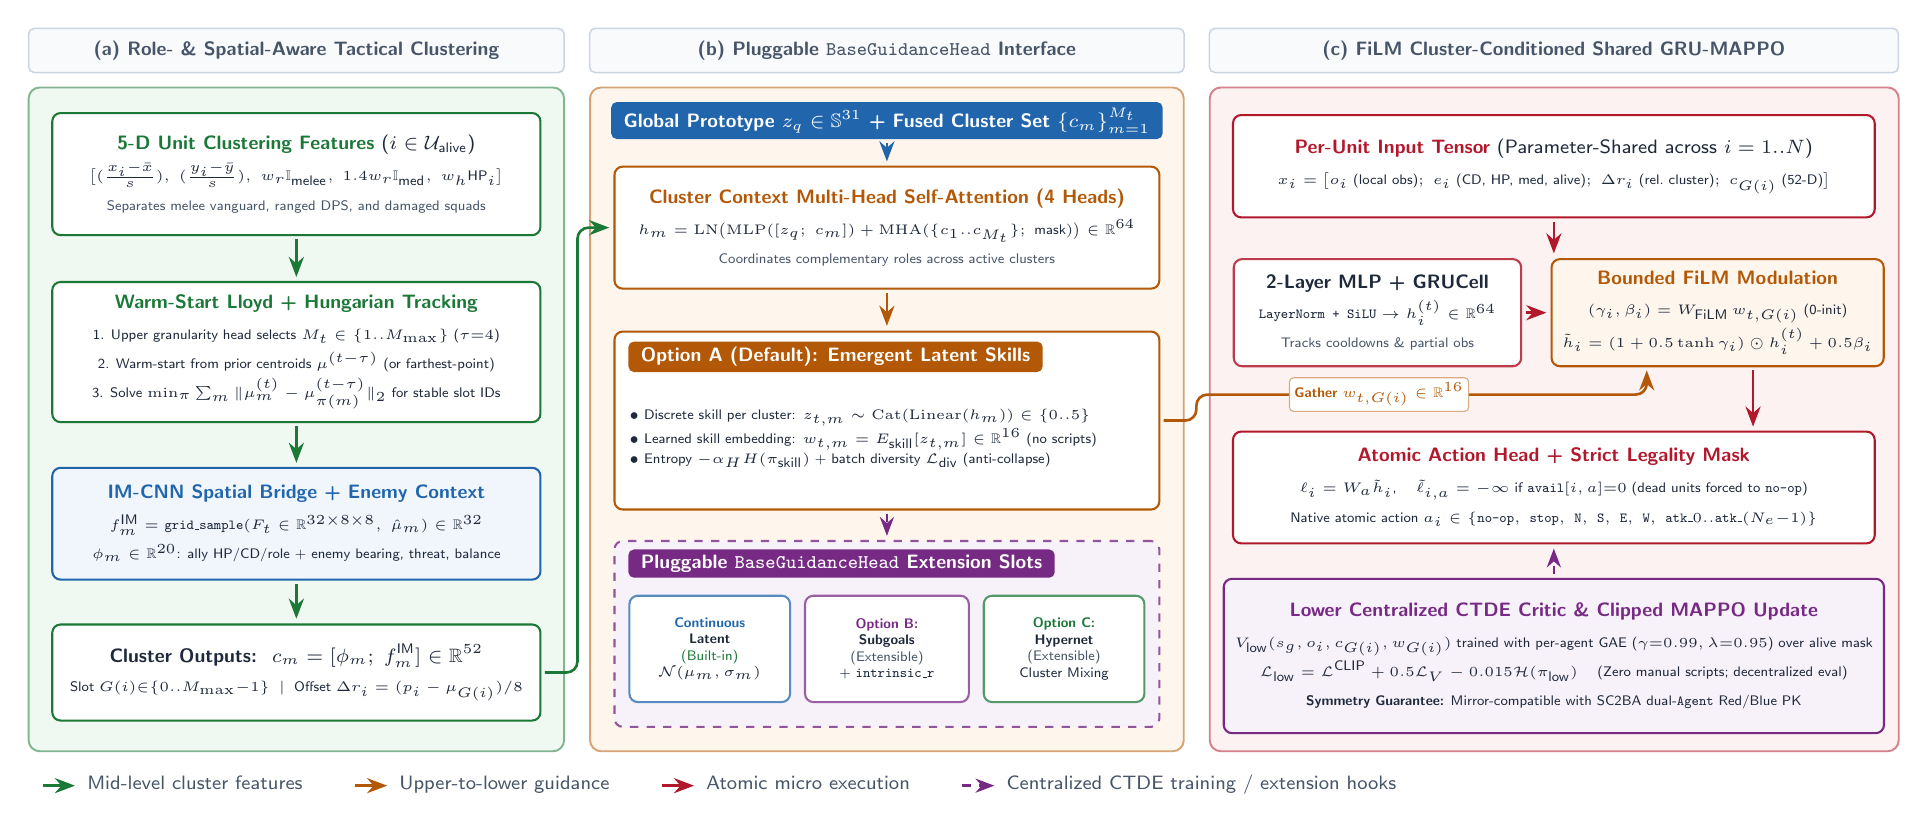
\begin{tikzpicture}[
  x=1cm, y=1cm,
  >=Stealth,
  font=\sffamily\footnotesize,
  box/.style={
    rectangle, rounded corners=3pt, draw=#1, fill=white,
    line width=0.75pt, align=center, inner sep=4pt, text=cInk
  },
  stagehdr/.style={
    rectangle, rounded corners=2pt, fill=cPanel, draw=cLine,
    line width=0.55pt, font=\sffamily\scriptsize\bfseries, text=cMuted,
    minimum height=0.56cm, align=center
  },
  pill/.style={
    rectangle, rounded corners=2pt, fill=#1, text=white,
    font=\sffamily\scriptsize\bfseries, inner xsep=4.5pt, inner ysep=2pt
  },
  flow/.style={->, line width=0.95pt, draw=#1, shorten >=1.5pt, shorten <=1.2pt},
  dashflow/.style={->, dashed, line width=0.85pt, draw=#1, shorten >=1.5pt, shorten <=1.2pt}
]

% 0. Top 3 Stage Banners & Background Zone Enclosures
\node[stagehdr, minimum width=6.80cm] at (3.45, 9.75) {(a) Role- \& Spatial-Aware Tactical Clustering};
\node[stagehdr, minimum width=7.55cm] at (10.95, 9.75) {(b) Pluggable \texttt{BaseGuidanceHead} Interface};
\node[stagehdr, minimum width=8.75cm] at (19.42, 9.75) {(c) FiLM Cluster-Conditioned Shared GRU-MAPPO};

\begin{scope}[on background layer]
  \filldraw[fill=cGreenBg,  draw=cGreen!55,  rounded corners=4pt, line width=0.7pt] (0.05, 0.85) rectangle (6.85, 9.28);
  \filldraw[fill=cOrangeBg, draw=cOrange!55, rounded corners=4pt, line width=0.7pt] (7.18, 0.85) rectangle (14.72, 9.28);
  \filldraw[fill=cRedBg,    draw=cRed!55,    rounded corners=4pt, line width=0.7pt] (15.05, 0.85) rectangle (23.80, 9.28);
\end{scope}

% 1. Zone (a): Role/Spatial Clustering
\node[box=cGreen, minimum width=6.20cm, minimum height=1.55cm] (FeatBox) at (3.45, 8.18) {
  {\scriptsize\textbf{\color{cGreen}5-D Unit Clustering Features} ($i \in \mathcal{U}_{\text{alive}}$)}\\[0.2em]
  {\tiny $\big[(\frac{x_i{-}\bar{x}}{s}),\; (\frac{y_i{-}\bar{y}}{s}),\; w_r\mathbb{I}_{\text{melee}},\; 1.4w_r\mathbb{I}_{\text{med}},\; w_h\text{HP}_i\big]$}\\[0.15em]
  {\tiny\color{cMuted}Separates melee vanguard, ranged DPS, and damaged squads}
};

\draw[flow=cGreen] (FeatBox.south) -- (3.45, 6.82);

\node[box=cGreen, minimum width=6.20cm, minimum height=1.78cm] (LloydBox) at (3.45, 5.92) {
  {\scriptsize\textbf{\color{cGreen}Warm-Start Lloyd + Hungarian Tracking}}\\[0.2em]
  {\tiny 1. Upper granularity head selects $M_t \in \{1..M_{\max}\}$ ($\tau{=}4$)}\\[0.1em]
  {\tiny 2. Warm-start from prior centroids $\mu^{(t-\tau)}$ (or farthest-point)}\\[0.1em]
  {\tiny 3. Solve $\min_\pi \sum_m \|\mu^{(t)}_m - \mu^{(t-\tau)}_{\pi(m)}\|_2$ for stable slot IDs}
};

\draw[flow=cGreen] (LloydBox.south) -- (3.45, 4.46);

\node[box=cBlue, fill=cBlueBg, minimum width=6.20cm, minimum height=1.42cm] (SpatialFuse) at (3.45, 3.74) {
  {\scriptsize\textbf{\color{cBlue}IM-CNN Spatial Bridge + Enemy Context}}\\[0.2em]
  {\tiny $f^{\text{IM}}_m = \texttt{grid\_sample}(F_t \in \mathbb{R}^{32\times 8\times 8},\; \hat{\mu}_m) \in \mathbb{R}^{32}$}\\[0.12em]
  {\tiny $\phi_m \in \mathbb{R}^{20}$: ally HP/CD/role + enemy bearing, threat, balance}
};

\draw[flow=cGreen] (SpatialFuse.south) -- (3.45, 2.48);

\node[box=cGreen, fill=white, minimum width=6.20cm, minimum height=1.22cm] (CluOut) at (3.45, 1.85) {
  {\scriptsize\textbf{\color{cInk}Cluster Outputs:}\; $c_m = [\phi_m;\; f^{\text{IM}}_m] \in \mathbb{R}^{52}$}\\[0.15em]
  {\tiny Slot $G(i){\in}\{0..M_{\max}{-}1\}$ \;\textbar\; Offset $\Delta r_i = (p_i - \mu_{G(i)})/8$}
};

% 2. Zone (b): Extensible BaseGuidanceHead Interface
\node[pill=cBlue] (ZqBadge) at (10.95, 8.86) {Global Prototype $z_q \in \mathbb{S}^{31}$ + Fused Cluster Set $\{c_m\}_{m=1}^{M_t}$};

\node[box=cOrange, minimum width=6.92cm, minimum height=1.55cm] (AttnBox) at (10.95, 7.50) {
  {\scriptsize\textbf{\color{cOrange}Cluster Context Multi-Head Self-Attention (4 Heads)}}\\[0.2em]
  {\tiny $h_m = \mathrm{LN}\big(\mathrm{MLP}([z_q;\; c_m]) + \mathrm{MHA}(\{c_1..c_{M_t}\};\; \text{mask})\big) \in \mathbb{R}^{64}$}\\[0.12em]
  {\tiny\color{cMuted}Coordinates complementary roles across active clusters}
};
\draw[flow=cBlue] (ZqBadge.south) -- (AttnBox.north);
\draw[flow=cGreen, rounded corners=4pt] (CluOut.east) -- (7.02, 1.85) -- (7.02, 7.50) -- (AttnBox.west);

\draw[flow=cOrange] (AttnBox.south) -- (10.95, 6.20);

\node[box=cOrange, fill=white, minimum width=6.92cm, minimum height=2.26cm] (OptA) at (10.95, 5.05) {};
\node[pill=cOrange, anchor=north west] at (7.66, 6.06) {Option A (Default): Emergent Latent Skills};
\node[font=\sffamily\tiny, text=cInk, align=left, text width=6.55cm] at (10.95, 4.82) {
  $\bullet$ Discrete skill per cluster: $z_{t,m} \sim \mathrm{Cat}(\mathrm{Linear}(h_m)) \in \{0..5\}$\\
  $\bullet$ Learned skill embedding: $w_{t,m} = E_{\text{skill}}[z_{t,m}] \in \mathbb{R}^{16}$ (no scripts)\\
  $\bullet$ Entropy $-\alpha_H H(\pi_{\text{skill}})$ + batch diversity $\mathcal{L}_{\text{div}}$ (anti-collapse)
};

\node[box=cPurple!80, fill=cPurpleBg, dashed, minimum width=6.92cm, minimum height=2.36cm] (ExtBox) at (10.95, 2.34) {};
\node[pill=cPurple, anchor=north west] at (7.66, 3.42) {Pluggable \texttt{BaseGuidanceHead} Extension Slots};

\node[box=cBlue!75, fill=white, minimum width=2.04cm, minimum height=1.35cm, inner sep=2.2pt, font=\sffamily\tiny] at (8.70, 2.15)
  {\textbf{\color{cBlue}Continuous}\\\textbf{Latent}\\{\color{cGreen}(Built-in)}\\$\mathcal{N}(\mu_m,\sigma_m)$};
\node[box=cPurple!75, fill=white, minimum width=2.08cm, minimum height=1.35cm, inner sep=2.2pt, font=\sffamily\tiny] at (10.95, 2.15)
  {\textbf{\color{cPurple}Option B:}\\\textbf{Subgoals}\\{\color{cMuted}(Extensible)}\\+ \texttt{intrinsic\_r}};
\node[box=cGreen!75, fill=white, minimum width=2.04cm, minimum height=1.35cm, inner sep=2.2pt, font=\sffamily\tiny] at (13.20, 2.15)
  {\textbf{\color{cGreen}Option C:}\\\textbf{Hypernet}\\{\color{cMuted}(Extensible)}\\Cluster Mixing};

\draw[dashflow=cPurple] (OptA.south) -- (ExtBox.north);

% 3. Zone (c): FiLM Shared GRU-Actor & CTDE Critic
\node[box=cRed, minimum width=8.15cm, minimum height=1.30cm] (UnitIn) at (19.42, 8.28) {
  {\scriptsize\textbf{\color{cRed}Per-Unit Input Tensor} (Parameter-Shared across $i = 1..N$)}\\[0.2em]
  {\tiny $x_i = \big[o_i\text{ (local obs)};\; e_i\text{ (CD, HP, med, alive)};\; \Delta r_i\text{ (rel.\ cluster)};\; c_{G(i)}\text{ (52-D)}\big]$}
};

\draw[flow=cRed] (UnitIn.south) -- (19.42, 7.12);

\node[box=cRed!85, minimum width=3.65cm, minimum height=1.36cm] (GRUBox) at (17.18, 6.42) {
  {\scriptsize\textbf{2-Layer MLP + GRUCell}}\\[0.15em]
  {\tiny \texttt{LayerNorm + SiLU} $\to h_i^{(t)} \in \mathbb{R}^{64}$}\\[0.1em]
  {\tiny\color{cMuted}Tracks cooldowns \& partial obs}
};

\node[box=cOrange, fill=cOrangeBg, minimum width=4.00cm, minimum height=1.36cm] (FiLMBox) at (21.50, 6.42) {
  {\scriptsize\textbf{\color{cOrange}Bounded FiLM Modulation}}\\[0.15em]
  {\tiny $(\gamma_i, \beta_i) = W_{\text{FiLM}}\, w_{t, G(i)}$ (0-init)}\\[0.1em]
  {\tiny $\tilde{h}_i = (1 + 0.5\tanh\gamma_i)\odot h_i^{(t)} + 0.5\beta_i$}
};
\draw[flow=cRed] (GRUBox.east) -- (FiLMBox.west);

% Clean guidance handoff from OptA -> FiLMBox south-west, leaving south-east clear for FiLM->ActBox!
\draw[flow=cOrange, rounded corners=4pt] (OptA.east) -- (14.88, 5.05) -- (14.88, 5.38) -- (20.60, 5.38) -- (20.60, 5.74);
\node[font=\sffamily\tiny\bfseries, text=cOrange, fill=white, draw=cOrange!50, rounded corners=1.5pt, inner sep=1.8pt]
  at (17.20, 5.38) {Gather $w_{t, G(i)} \in \mathbb{R}^{16}$};

\draw[flow=cRed] (21.95, 5.74) -- (21.95, 4.92);

\node[box=cRed, minimum width=8.15cm, minimum height=1.42cm] (ActBox) at (19.42, 4.20) {
  {\scriptsize\textbf{\color{cRed}Atomic Action Head + Strict Legality Mask}}\\[0.2em]
  {\tiny $\ell_i = W_a \tilde{h}_i$, \quad $\tilde{\ell}_{i,a} = -\infty$ if $\texttt{avail}[i,a]{=}0$ (dead units forced to \texttt{no-op})}\\[0.12em]
  {\tiny Native atomic action $a_i \in \{\texttt{no-op},\;\texttt{stop},\;\texttt{N},\;\texttt{S},\;\texttt{E},\;\texttt{W},\;\texttt{atk\_}0..\texttt{atk\_}(N_e{-}1)\}$}
};

\node[box=cPurple, fill=cPurpleBg, minimum width=8.15cm, minimum height=1.96cm] (CriticBox) at (19.42, 2.06) {
  {\scriptsize\textbf{\color{cPurple}Lower Centralized CTDE Critic \& Clipped MAPPO Update}}\\[0.2em]
  {\tiny $V_{\text{low}}(s_g, o_i, c_{G(i)}, w_{G(i)})$ trained with per-agent GAE ($\gamma{=}0.99, \lambda{=}0.95$) over alive mask}\\[0.12em]
  {\tiny $\mathcal{L}_{\text{low}} = \mathcal{L}^{\text{CLIP}} + 0.5\mathcal{L}_V - 0.015\mathcal{H}(\pi_{\text{low}})$ \quad (Zero manual scripts; decentralized eval)}\\[0.12em]
  {\tiny\color{cInk}\textbf{Symmetry Guarantee:} Mirror-compatible with SC2BA dual-\texttt{Agent} Red/Blue PK}
};
\draw[dashflow=cPurple] (CriticBox.north) -- (ActBox.south);

\node[font=\sffamily\scriptsize, text=cMuted, anchor=west] at (0.05, 0.42) {
  \tikz[baseline=-0.5ex]{\draw[flow=cGreen] (0,0)--(0.50,0);} Mid-level cluster features \qquad
  \tikz[baseline=-0.5ex]{\draw[flow=cOrange] (0,0)--(0.50,0);} Upper-to-lower guidance \qquad
  \tikz[baseline=-0.5ex]{\draw[flow=cRed] (0,0)--(0.50,0);} Atomic micro execution \qquad
  \tikz[baseline=-0.5ex]{\draw[dashflow=cPurple] (0,0)--(0.50,0);} Centralized CTDE training / extension hooks
};

\end{tikzpicture}
\end{document}
